\documentclass[10pt,aspectratio=169]{beamer}
\usetheme{metropolis}
\usecolortheme{owl} % Sleek dark theme suitable for quant pitch decks

\usepackage{booktabs}
\usepackage{graphicx}

\title{\textbf{Nonlinear Liquidity Reversion (NLR) Strategy}}
\subtitle{Execution Horizon \& Capacity Analysis}
\author{\textbf{Quantitative Research Division} \\ Confidential -- Proprietary Research}
\date{July 2026}

\begin{document}

\maketitle

% Slide 1
\begin{frame}{1. Executive Summary}
    \begin{itemize}
        \item \textbf{Objective:} Systematic capture of overnight overreaction anomalies in US Small/Micro-Cap Equities.
        \item \textbf{Performance (2020--2026):} Net Sharpe Ratio of \textbf{1.492}, CAGR of \textbf{91.04\%}, Max Drawdown of -57.45\%.
        \item \textbf{Leverage:} 1.0x (No borrowing interest drag, zero margin call risk).
        \item \textbf{Capacity Ceiling:} Scalable up to \textbf{\$2.5M -- \$3.0M AUM}.
        \item \textbf{Key Insight:} Slippage mitigation via a 3-hour VWAP execution horizon is the primary driver of compounding returns.
    \end{itemize}
\end{frame}

% Slide 2
\begin{frame}{2. The Anomaly: Overnight Overreaction}
    \begin{itemize}
        \item \textbf{Economic Intuition:} Intraday extreme flows push prices past fair value due to daytime liquidity concentration.
        \item \textbf{Market Maker Premium:} Liquidity providers demand a return premium for holding inventory overnight.
        \item \textbf{Overnight Reversion:} Institutional imbalances and retail momentum mean-revert during the Close-to-Open session.
        \item \textbf{The Alpha Pool:} Most pronounced in micro-cap stocks where capital flows trigger disproportionate price dislocations.
    \end{itemize}
\end{frame}

% Slide 3
\begin{frame}{3. Signal Construction \& Filtering}
    \begin{itemize}
        \item \textbf{Signal Input:} Cross-sectional long-only equity rank based on intraday mid-price deviation from Close.
        \item \textbf{Top-N Focus:} Highly concentrated in the **Top 4** alpha-ranked stocks daily.
        \item \textbf{Dynamic Liquidity Filter:}
            \begin{itemize}
                \item AUM < \$100K: **\$50K ADDV soft floor** (protects fills, avoids nano-caps).
                \item AUM $\ge$ \$100K: **\$1M ADDV floor** (mitigates slippage).
            \end{itemize}
    \end{itemize}
\end{frame}

% Slide 4
\begin{frame}{4. Portfolio Architecture: Tranche Rebalancing}
    \begin{itemize}
        \item \textbf{Turnover Bottleneck:} Daily rebalancing triggers heavy commission and execution slippage drag.
        \item \textbf{Tranche Solution:} Position split across 3 independent daily tranches.
        \item \textbf{Holding Period:} Each tranche holds positions for **3 days**.
        \item \textbf{Mathematical Impact:} Reduces daily traded volume and turnover by **67\%**, preserving capacity at scale.
    \end{itemize}
\end{frame}

% Slide 5
\begin{frame}{5. The Execution Horizon Tradeoff}
    Slicing entry/exit trades balances market impact reduction against morning-session alpha decay:
    \begin{equation*}
        \text{Net Return}(H) = \text{Gross Alpha} - a \cdot H - \frac{b}{H}
    \end{equation*}
    Taking the second derivative verifies strict concavity:
    \begin{equation*}
        \frac{d^2(\text{Net Return})}{dH^2} = -\frac{2b}{H^3} < 0
    \end{equation*}
    \begin{itemize}
        \item \textbf{Inflection Point:} Peak net return is achieved at **$H^* = 3.0$ hours**.
        \item \textbf{Operational Window:} Exits sliced via a 3-hour VWAP from 9:30 AM to 12:30 PM EST.
    \end{itemize}
\end{frame}

% Slide 6
\begin{frame}{6. Capacity scaling curve (1998--2026)}
    \begin{table}
        \centering
        \caption{Performance Net of Slippage, Commissions, and Spreads}
        \begin{tabular}{lcccc}
            \toprule
            AUM Scale & Net Sharpe & Net CAGR & Max Drawdown & Execution Safety \\
            \midrule
            \$10K & 2.571 & 386.36\% & -48.07\% & Safe \\
            \$100K & 1.652 & 96.12\% & -55.19\% & Safe \\
            \$1.0M & 1.463 & 79.34\% & -57.45\% & Safe \\
            \$2.5M & 1.303 & 66.21\% & -64.44\% & Terminal \\
            \$10.0M & 0.866 & 35.13\% & -78.20\% & Over-capacity \\
            \bottomrule
        \end{tabular}
    \end{table}
\end{frame}

% Slide 7
\begin{frame}{7. Strategy Equity Curve (PnL)}
    \begin{figure}
        \centering
        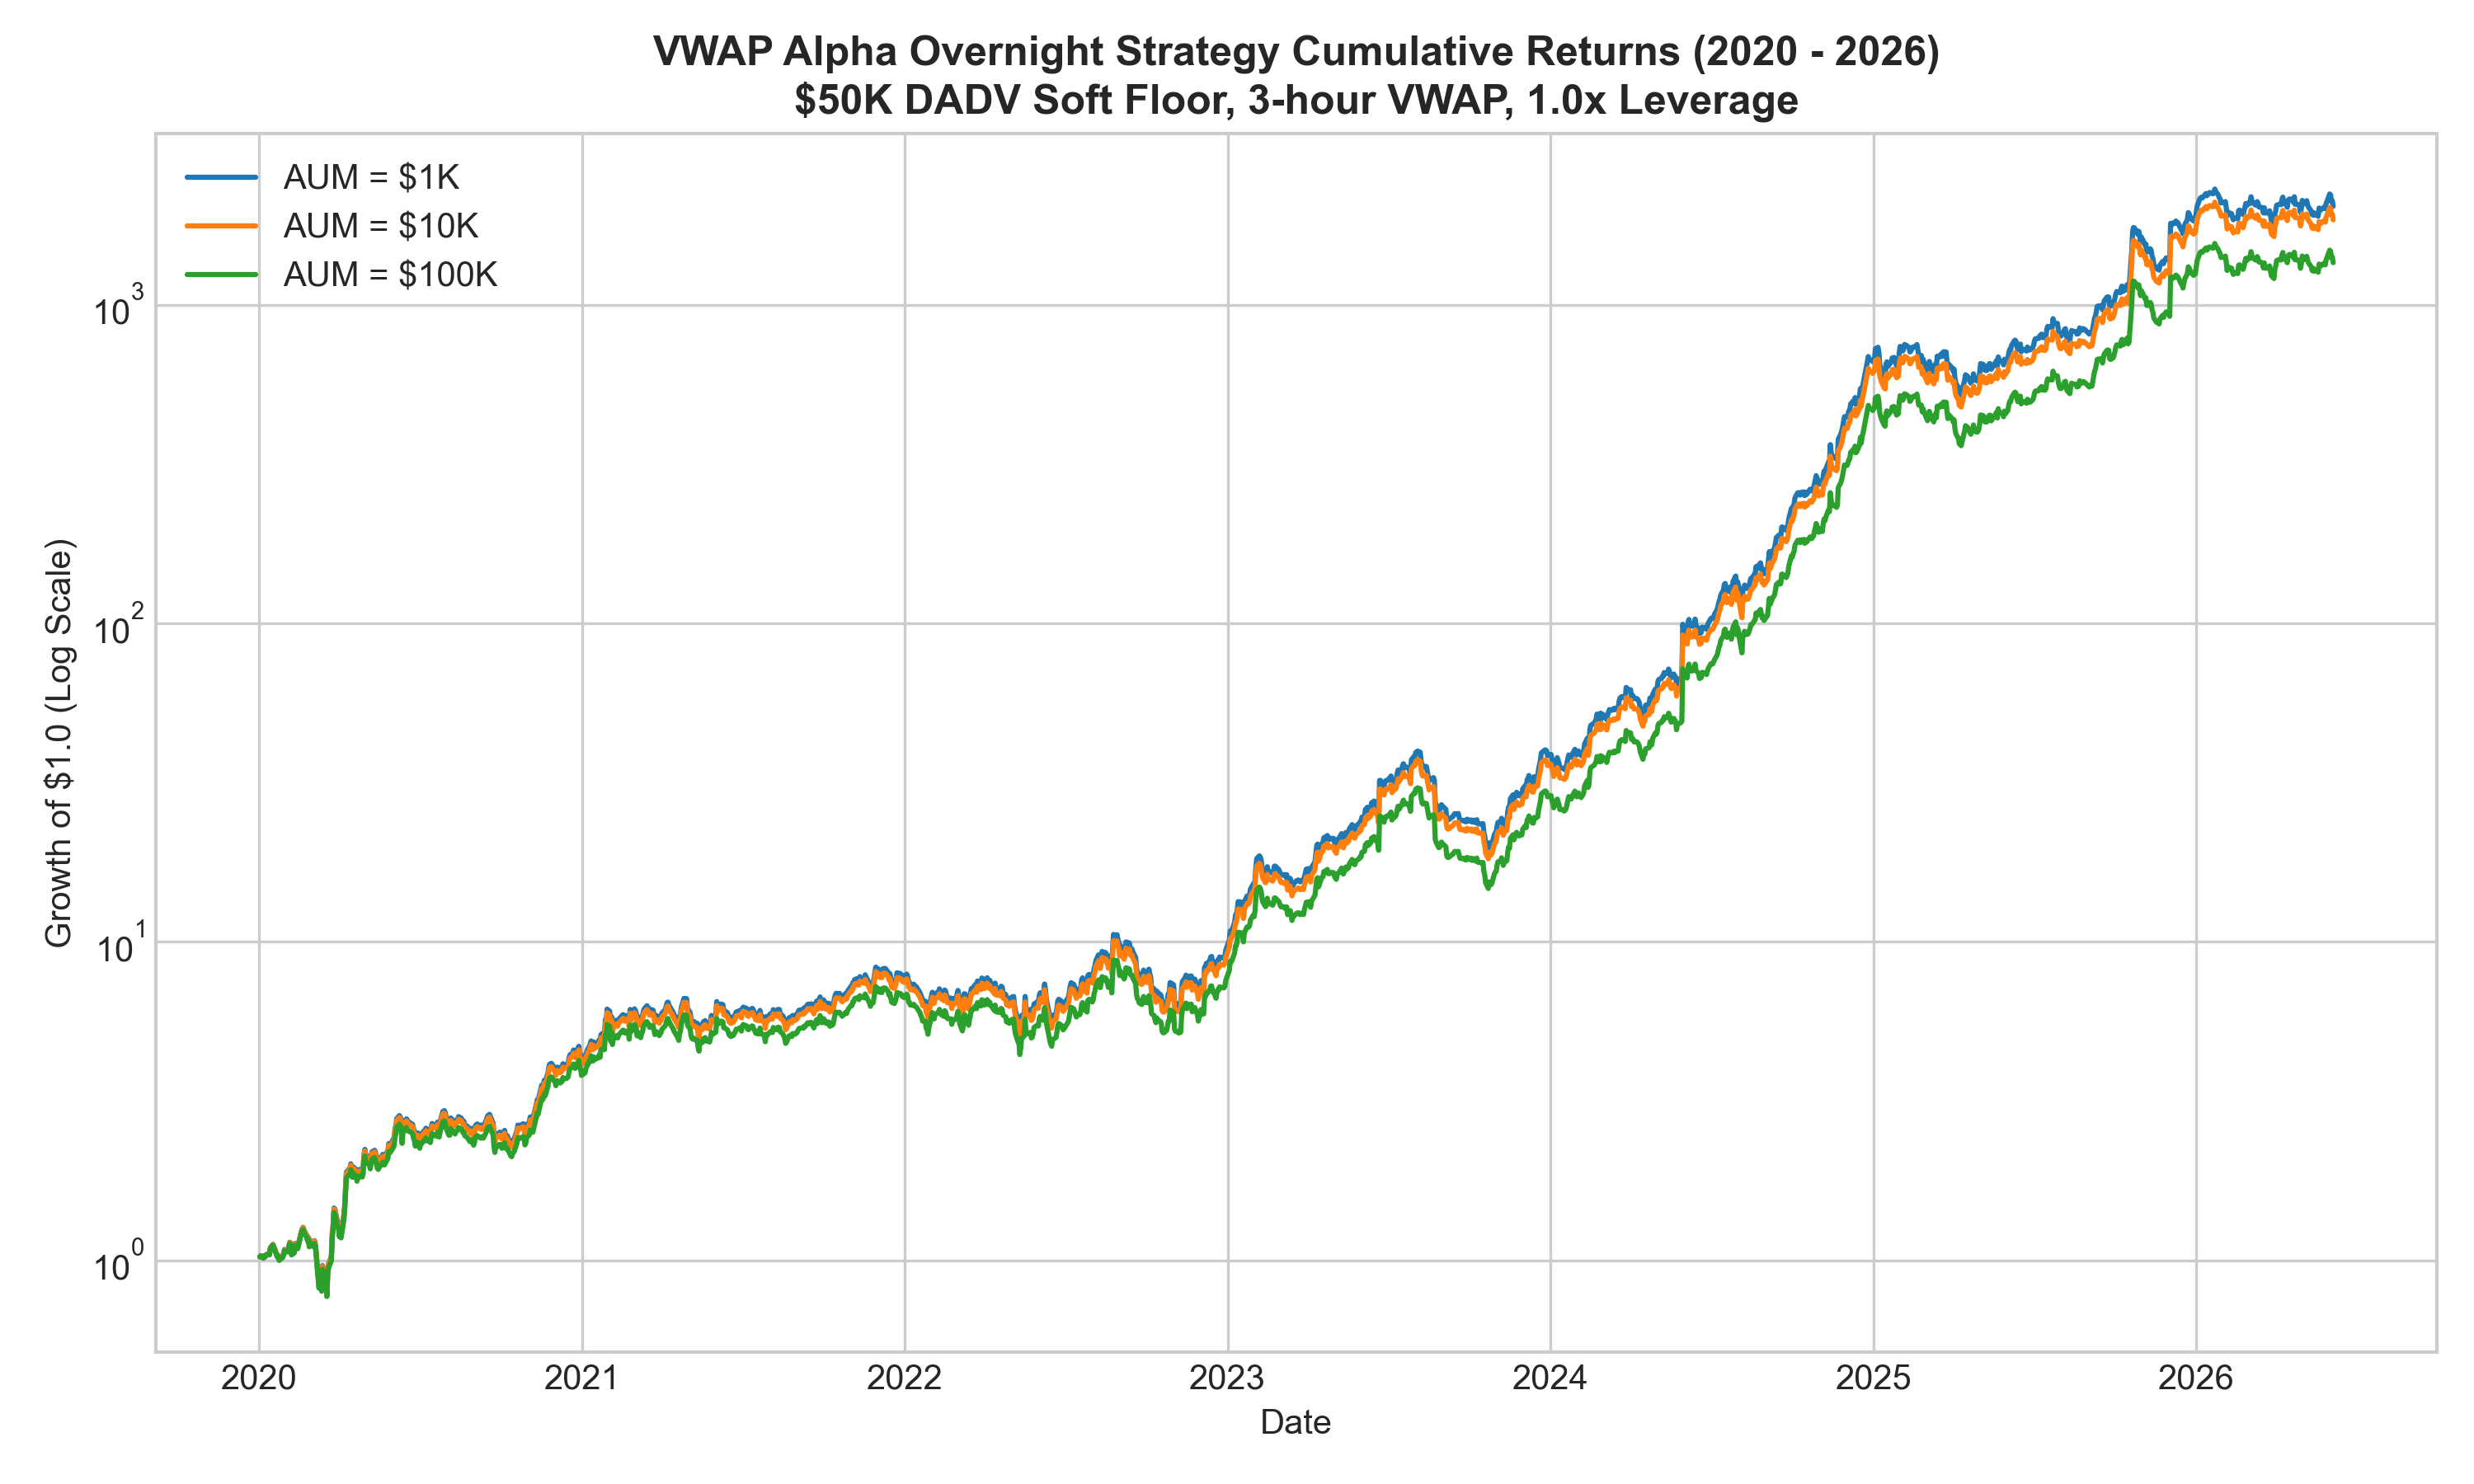
\includegraphics[width=0.7\textwidth]{pnl_chart_2020_2026.png}
        \caption{Growth of \$1.0 invested since Jan 2020 (Log Scale)}
    \end{figure}
\end{frame}

% Slide 8
\begin{frame}{8. Sub-Period Robustness Regimes}
    \begin{table}
        \centering
        \caption{Net Sharpe Ratios across Historical Sub-Periods}
        \begin{tabular}{lcccc}
            \toprule
            AUM Scale & Pre-Crisis (1998-2007) & Post-Crisis (2008-2019) & COVID/Modern (2020-2026) & Full Horizon \\
            \midrule
            \$10K & 3.348 & 2.230 & 2.355 & 2.560 \\
            \$1.0M & 1.964 & 1.126 & 1.466 & 1.462 \\
            \$3.0M & 1.744 & 0.903 & 1.299 & 1.260 \\
            \$5.0M & 1.593 & 0.750 & 1.184 & 1.120 \\
            \bottomrule
        \end{tabular}
    \end{table}
\end{frame}

% Slide 9
\begin{frame}{9. Key Risk Control Parameters}
    \begin{itemize}
        \item \textbf{Inverse Volatility Weighting:} Assets allocated proportional to $1/\sigma_i$ (delivers a 27\% utility boost over EW).
        \item \textbf{Market Trend Guardrail:} halt all trading when S\&P 500 falls below its 200-day simple moving average.
        \item \textbf{Compounding Cap:} Halt strategy compounding once account equity reaches \$2.5M. Daily net realized gains are swept monthly as idle cash.
    \end{itemize}
\end{frame}

% Slide 10
\begin{frame}{10. Conclusion \& Implementation Roadmap}
    \begin{itemize}
        \item \textbf{Viability:} Strategy is highly scalable to \$2.5M AUM.
        \item \textbf{Starting Capital:} Recommend \$10K minimum to dilute ticket commissions.
        \item \textbf{Broker Implementation:} Deploy via IBKR Pro API Gateway.
        \item \textbf{Order Routing:} Utilise native IBKR VWAP algorithm scheduled for 3-hour execution.
    \end{itemize}
\end{frame}

\end{document}
